\section{State-transition System}




%A restricted state-transition system is one that meets all of the restrictive assumptions
%A0 through A7 given in Chapter 1. It is a deterministic, static, finite, and fully
%observable state-transition system with restricted goals and implicit time. Such a
%system is denoted E--(S,A, F) instead of (S,A, E, Y) because there are no contingent
%events. Here S, A, and Y are finite, and y(s, a) is a single state when a is
%applicable to s.
%A planning problem for a restricted state-transition system E--(S,A, F) is
%defined as a triple P = (E, so, g), where so is an initial state and g corresponds to a
%set of goal states. A solution to P is a sequence of actions (al, a2 . . . . . ak) correspondingto
%a sequence ofstate transitions (so, Sl,..., Sk) such that Sl = Y(so, a l ) , . . . , Sk -
%y(Sk-l,ak), and Sk is a goal state. The planning problem is to synthesize such a
%sequence of actions.
%Classical planning refers generically to planning for restricted state-transition
%systems.



A state-transition system is a 4-tuple  $\sum = (\mathsf{S},\mathsf{A},\mathsf{E},\gamma)$
\begin{itemize}
\item $\mathsf{S}=\lbrace s_1,s_2, \dots\rbrace$ is a finite or recursively enumerable set of states;
\item $\mathsf{A}=\lbrace a_1,a_2, \dots\rbrace$ is a finite or recursively enumerable set of actions;
\item $\mathsf{E}=\lbrace e_1,e_2, \dots\rbrace$ is a finite or recursively enumerable set of events;
\item $\gamma:\mathsf{S} \times \mathsf{A} \times \mathsf{E} \to 2^\mathsf{S}$
\end{itemize}

\begin{figure}[h!]
\begin{center}
$
\psmatrix[colsep=4cm,rowsep=1cm,mnode=circle]
[linecolor=MidnightBlue]s_0 &s_{11}&s_{12}\\
s_{1}&s_{10}&s_{13}\\
s_{2}&s_{9}&s_{14}\\
s_{3}&s_{8}&s_{15}\\
s_{4}&s_{7}&[linecolor=RubineRed]s_{16}\\
s_{5}&s_{6}
\ncarc[arcangle=-30]{->}{1,1}{2,1}<{attach}
\ncarc[arcangle=30]{<-}{1,1}{2,1}>{remove}
\ncline{->}{2,1}{3,1}<{aboveBekt}
\ncline{->}{3,1}{4,1}<{takeEkt}
\ncline{->}{4,1}{5,1}<{putEkt}
\ncline{->}{5,1}{6,1}<{remove}
\ncline{->}{6,1}{6,2}^{attach}
\ncline{->}{6,2}{5,2}>{aboveP}
\ncline{->}{5,2}{4,2}>{takeP}
\ncline{->}{4,2}{3,2}>{aboveKit}
\ncline{->}{3,2}{2,2}>{putP}
\ncarc[arcangle=-30]{->}{2,2}{5,2}<{aboveP}
\ncline{->}{2,2}{1,2}>{remove}
\ncline{->}{1,2}{1,3}^{attach}
\ncline{->}{1,3}{2,3}<{aboveKit}
\ncline{->}{2,3}{3,3}<{takeFkt}
\ncline{->}{3,3}{4,3}<{aboveBfkt}
\ncline{->}{4,3}{5,3}<{putFkt}
\endpsmatrix
$
\end{center}
\caption{\label{fig:state_transition}A state-transition system for the kitting domain.}
\end{figure}

A state-transition system may be represented by a directed graph whose nodes are
the states in $S$. If $s\prime \in \gamma(s,u)$, where $u$ is a pair $(a, e)$, $a \in A$ and $e \in E$, then the graph contains an arc from $s$ to $s\prime$ that is labeled with $u$. Each such arc is called a
state transition.\\ \\
Figure~\ref{fig:state_transition} shows a state-transition system for the kitting environment with $s_0$ as the initial state and $s_{16}$ as the goal state.
\begin{comment}
Figure~\ref{fig:state0} depicts the status of the workstation in state $s_0$.
\begin{figure}[h!]
\centering
\resizebox{\columnwidth}{!}{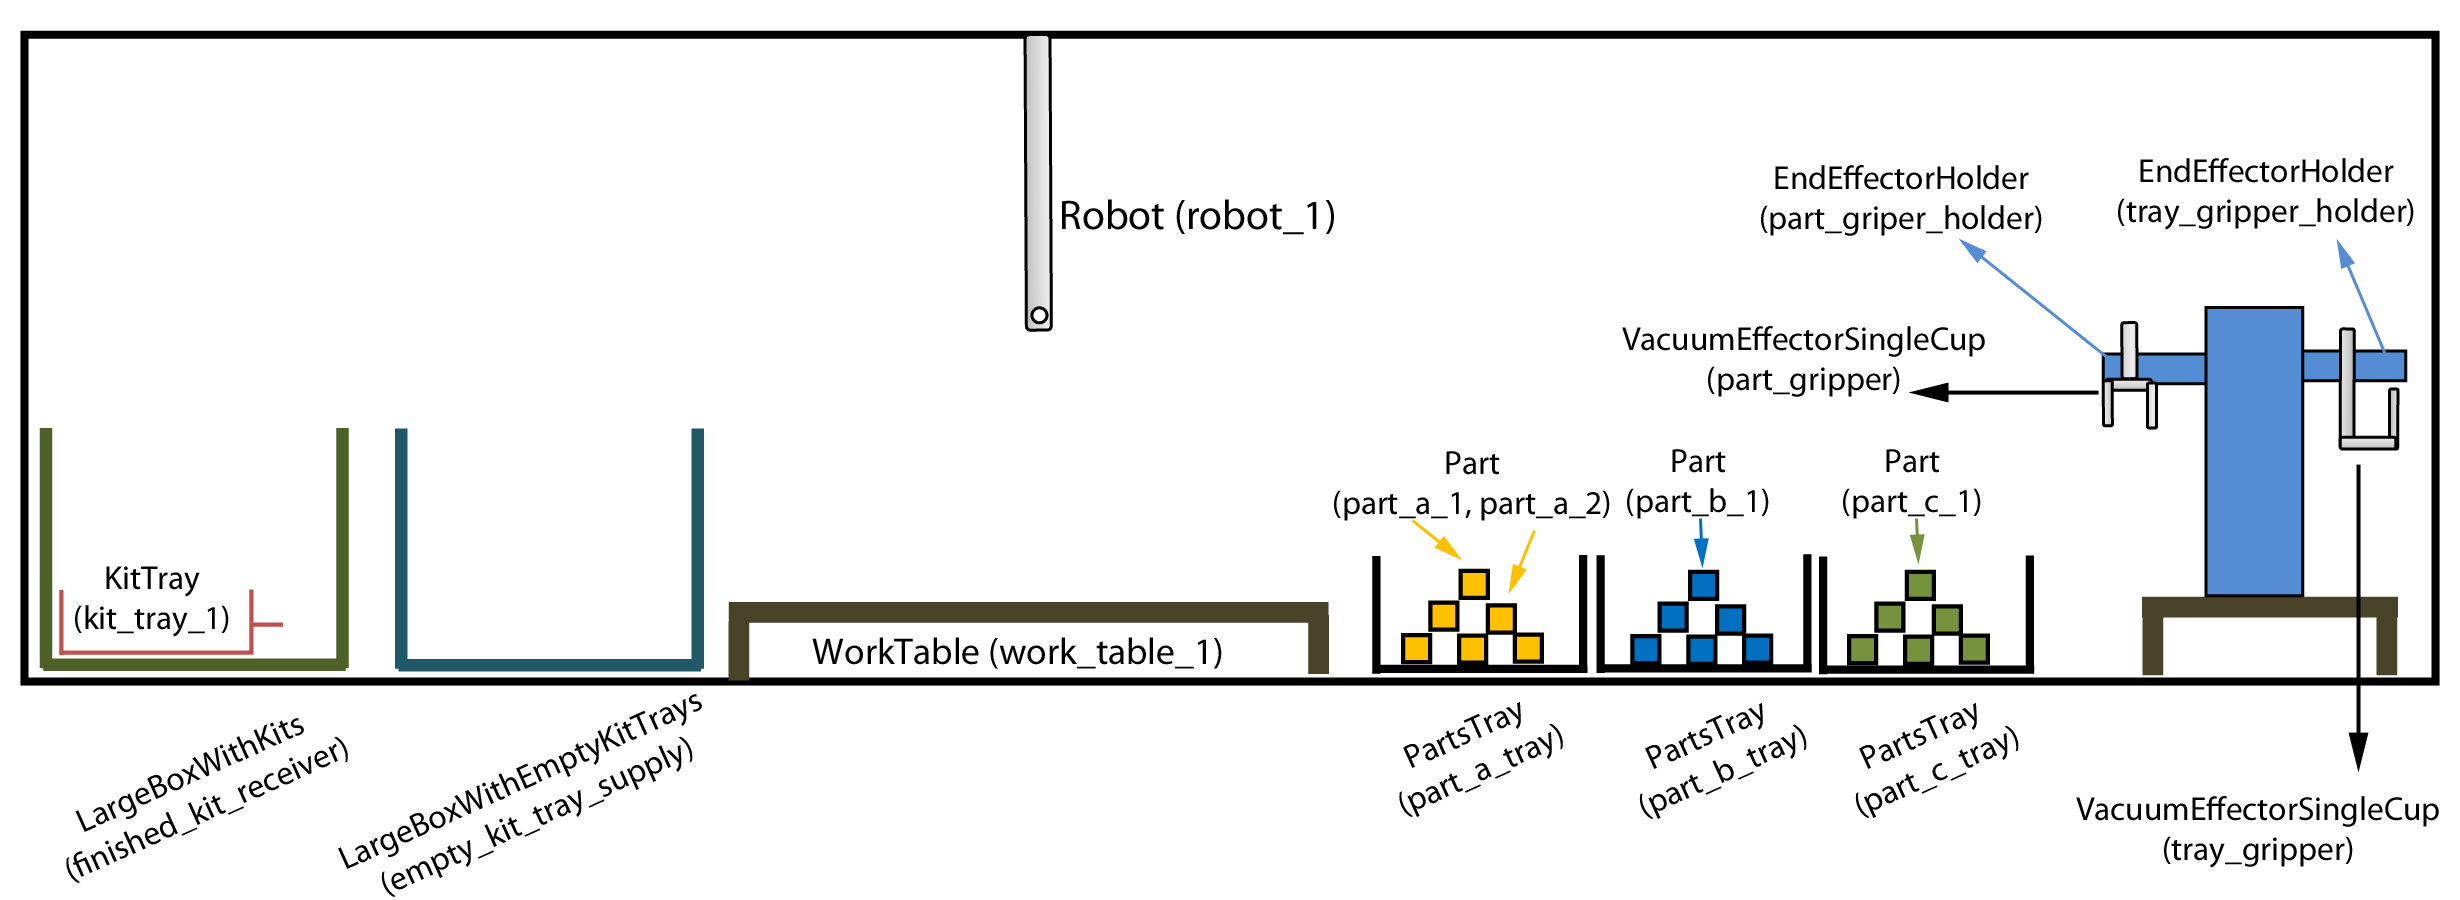
\includegraphics[width=8cm]{s0.eps}}
\caption{\label{fig:state0}Initial status of the workstation.}
\end{figure}
\end{comment} 